%%%%%%%%%%%%%%%%%%%%%%%%%%%%%%%%%%%%%%%%%%%%%%%%%%%%%%%%%%%%%%%%%%%%%%%%%%%%%%%
%% StuPro B, "Programmierumgebung Offener Antrieb" (POA)
%% Handbuch Tutorial
%% $Id: tutorial.tex,v 1.3 2004/03/18 13:48:16 neco Exp $
%% Achtung: Diese Datei wird in das Handbuch inkludiert!
%%%%%%%%%%%%%%%%%%%%%%%%%%%%%%%%%%%%%%%%%%%%%%%%%%%%%%%%%%%%%%%%%%%%%%%%%%%%%%%

\chapter {Tutorial}
Um dem Benutzer einen leichten Einstieg in POA zu verschaffen, wird in diesem Kapitel ein POA-Projekt anhand eines einfachen Regelkreises f"ur eine Antriebsregelung realisiert. Die Abbildung 4.1 gibt alle n"otigen Daten f"ur das Projekt wieder.
\begin{figure}[htbp]

\begin{center}

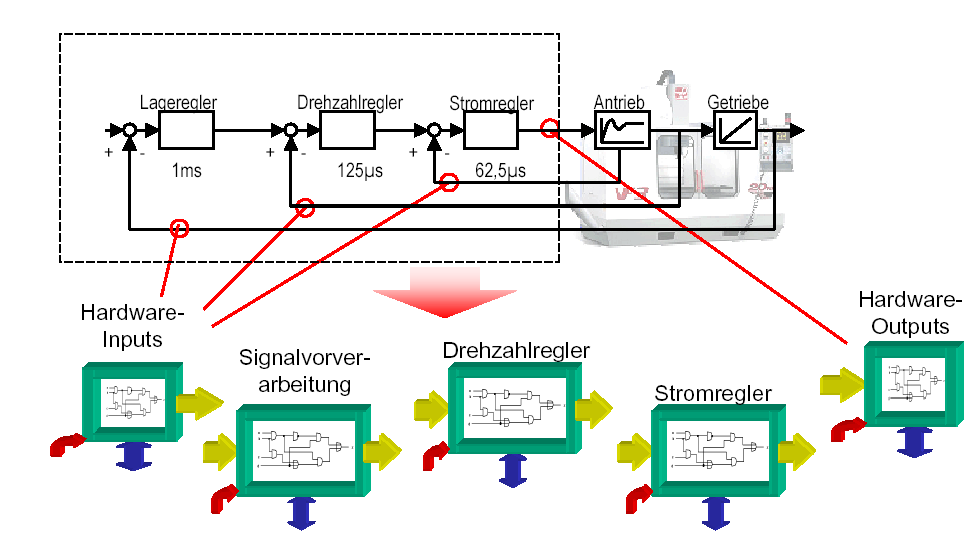
\includegraphics[width=15cm]{Beispielsprojekt}
\caption{Beispielsprojekt}\label{test}
\end{center}

\end{figure}
\newline
Standard Regelkreis:
\begin{itemize}
	\item Lageregler: Eing"ange {\itshape xSoll[32], xIst[32]} und Ausgang {\itshape nSoll[32]}
	\item Drehzahlregler: Eing"ange {\itshape nSoll[32], nIst[32]} und Ausgang {\itshape iSoll[10]}
	\item Stromregler: Eing"ange {\itshape iSoll[10], iIst[10]} und Ausgang {\itshape stell[10]}
\end{itemize}

Zus"atzlich:
\begin{itemize}
	\item Signalvorverabeitung: Eing"ange {\itshape xIst-raw, nIst-raw, iIst-raw} und Ausg"ange {\itshape xIst[32], nIst[32], iIst[10]}
	\item HardwareInputs: Ausg"ange {\itshape xIst-raw, nIst-raw, iIst-raw}
	\item HardwareOutput: Eingang {\itshape stell[10]}
\end{itemize}
Die Zahlen in den eckigen Klammer geben die Bitbreite an.
\par

\section {Beispielprojekt  anlegen}
Bevor man mit dem Layout f"ur den Antriebsregler anfangen kann, muss zun"achts einmal das Projekt angelegt werden. Dazu muss man folgenderma"sen vorgehen:
\begin{enumerate}
	\item In der Menleiste {\bf Project} den Eintrag {\bf New} ausw"ahlen
	\item Im Dialog {\bf Select/Create project directory} den gew"unschten Pfad angeben
	\item Den Button {\bf Create New Directory} anklicken
	\item Name des Projekt eingeben und mit Return best"atigen
	\item Den neu erzeugten Ordner anw"ahlen und den Button {\bf Open} dr"ucken
	\item Die Datei {\bf project.xlm} anw"ahlen und den Button {\bf Open} dr"ucken
\end{enumerate}
Nach dem Anlegen und "offnen des neuen Projekt wird das Arbeitsfenster mit einem leeren Layout ge"offnet.
\section{Funktionsbl"ocke erzeugen und konfigurieren}
Zur Realisierung des Antriebreglers ben"otigt man verschiedene Typen von Bl"ocken und zwar:
\begin{itemize}
	\item 2 I/O-Bl"ocke, einen f"ur HardwareInput und einen f"ur HardwareOutput
	\item 3 CPU-Bl"ocke f"ur Signalverarbeitung, Drehzahlregler und Lageregler
	\item 1 Core-Block f"ur Stromregler
\end{itemize}
\subsection{HardwareInput- und HardwareOutput-Block}
HardwareInput- und HardwareOutput-Block bilden die Schnittstelle nach Au"sen. Daher werden I/O-Blcke verwendet. Die ankommenden Signale werden "uber den HardwareInput-Block an den Singalverarbeitungsblock weitergeleitet. Signale, die nach Au"sen weitergeleitet werden m"ussen, kommen in den HardwareOutput-Block. Als erstes wird der HardwareInput erzeugt und konfiguriert:
\begin{enumerate}
	\item Einen I/O-Block aus der Blockbiliothek per Drag'n Drop ziehen, d.h. mit dem Mauszeiger den Block ankilcken, die Maustaste dabei gedr"uckt lassen, den Block ins Arbeitsfenster ziehen und die Maustaste wieder loslassen.
	\item Im Dialog {\bf Block configuration} als erstes den Namen {\itshape "'HardwareInput"'} eingeben
	\item Unter {\bf Description} den Block beschreiben {\itshape "'..."uber diesen Inputblock werden die Signale weitergeleitet..."'}
	\item Den Offset Eintrag auf {\itshape "'Auto (0 ns)"'} lassen
	\item Unter {\bf Clock} den Takt f"ur den Block angeben, d.h. {\itshape "'62,5 ns"'}
	\item Pins konfigurieren fr die 4 Ausg"ange:
		\begin{itemize}
			\item Pinnamen angeben
			\item Bitbreite angeben
			\item Adresse angeben
		\end{itemize}
\end{enumerate}
